%Title of section

\begin{frame}
\frametitle{研究目标}
\begin{block}{解决CaaS模式下云数据中心的能耗优化问题}
    \begin{itemize}
        \item 负载预测模型
        \begin{itemize}
            \item 实时性
            \item 主动资源配置和容器调度
        \end{itemize}
        \item 基于负载状态容器调度策略
        \begin{itemize}
            \item 保证云服务QoS(Quality of Service)
            \item 降低整体能耗
        \end{itemize}
    \end{itemize}
\end{block}
\end{frame}

\subsection{研究目标}

\subsubsection{容器负载预测模型}

\begin{frame}
\frametitle{研究目标}
\framesubtitle{目标1:容器负载预测模型
\onslide*<1-2>{$\Rightarrow$ \textbf{单值预测模型}}
\onslide*<3-4>{$\Rightarrow$ \textbf{区间预测模型}}}
\onslide*<1,3>{
\begin{block}{负载预测模型}
\begin{itemize}
    \item<1-1> 单值预测模型:预测负载的特定值
    \begin{itemize}
        \item<1-1> \textbf{误差敏感} $\Rightarrow$ \textbf{决策失效}
        \item<1-1> \textbf{鲁棒性差} $\Rightarrow$ \textbf{决策过度}
    \end{itemize}
    \item<3-3> 区间预测模型\textsuperscript{$\star$}:预测负载的取值区间
\end{itemize}
\end{block}
}
\onslide*<1>{
\begin{table}[hftb]
\centering
\resizebox{0.7\textwidth}{!}{%
    \begin{tabular}{ccl}
        \toprule
        \textbf{类型} & \textbf{模型名称} & \textbf{简述}\\
        \midrule
        \multirow{4}{*}{统计学模型} & ARIMA & 差分自回归移动平均\\
        ~ & Kalman滤波 & 基于递推演进和观测值对预测结果进行演进\\
        ~ & 排队论模型 & 基于在线作业请求和系统阻塞情况进行预测\\
        ~ & 灰色模型 & 模型新陈代谢过程,进行中长期预测\\
        \midrule
        \multirow{4}{*}{机器学习模型} & RNN & 递归神经网络预测\\
        ~ & BPNN & 原始信息前向传播,误差信息后向传播\\
        ~ & LSTM & 长短期记忆网络\\
        ~ & 混合模型 & 基于c-means聚类和模糊(Fuzzy)神经网络\\
        \bottomrule
    \end{tabular}
}
\caption{单值预测模型}
\label{tab:tab1}
\end{table}
}

\onslide*<3>{
\begin{table}[hftb]
    \centering
    \resizebox{0.7\textwidth}{!}{%
        \begin{tabular}{ccl}
            \toprule
            \textbf{类型} & \textbf{模型名称} & \textbf{简述}\\
            \midrule
            概率论模型 & 贝叶斯模型 & 根据样本分布假设和统计学特征扩展区间\\
            \midrule
            \multirow{4}{*}{机器学习模型} & 线性回归 & \multirow{4}{*}{先拟合单值再根据分布假设构建区间}\\
            ~ & SVM & \\
            ~ & CART & \\
            ~ & 随机森林 & \\
            \bottomrule
        \end{tabular}
    }
    \caption{区间预测模型}
    \label{tab:tab2}
    \end{table}
}

\onslide*<2>{
\begin{figure}[htb]
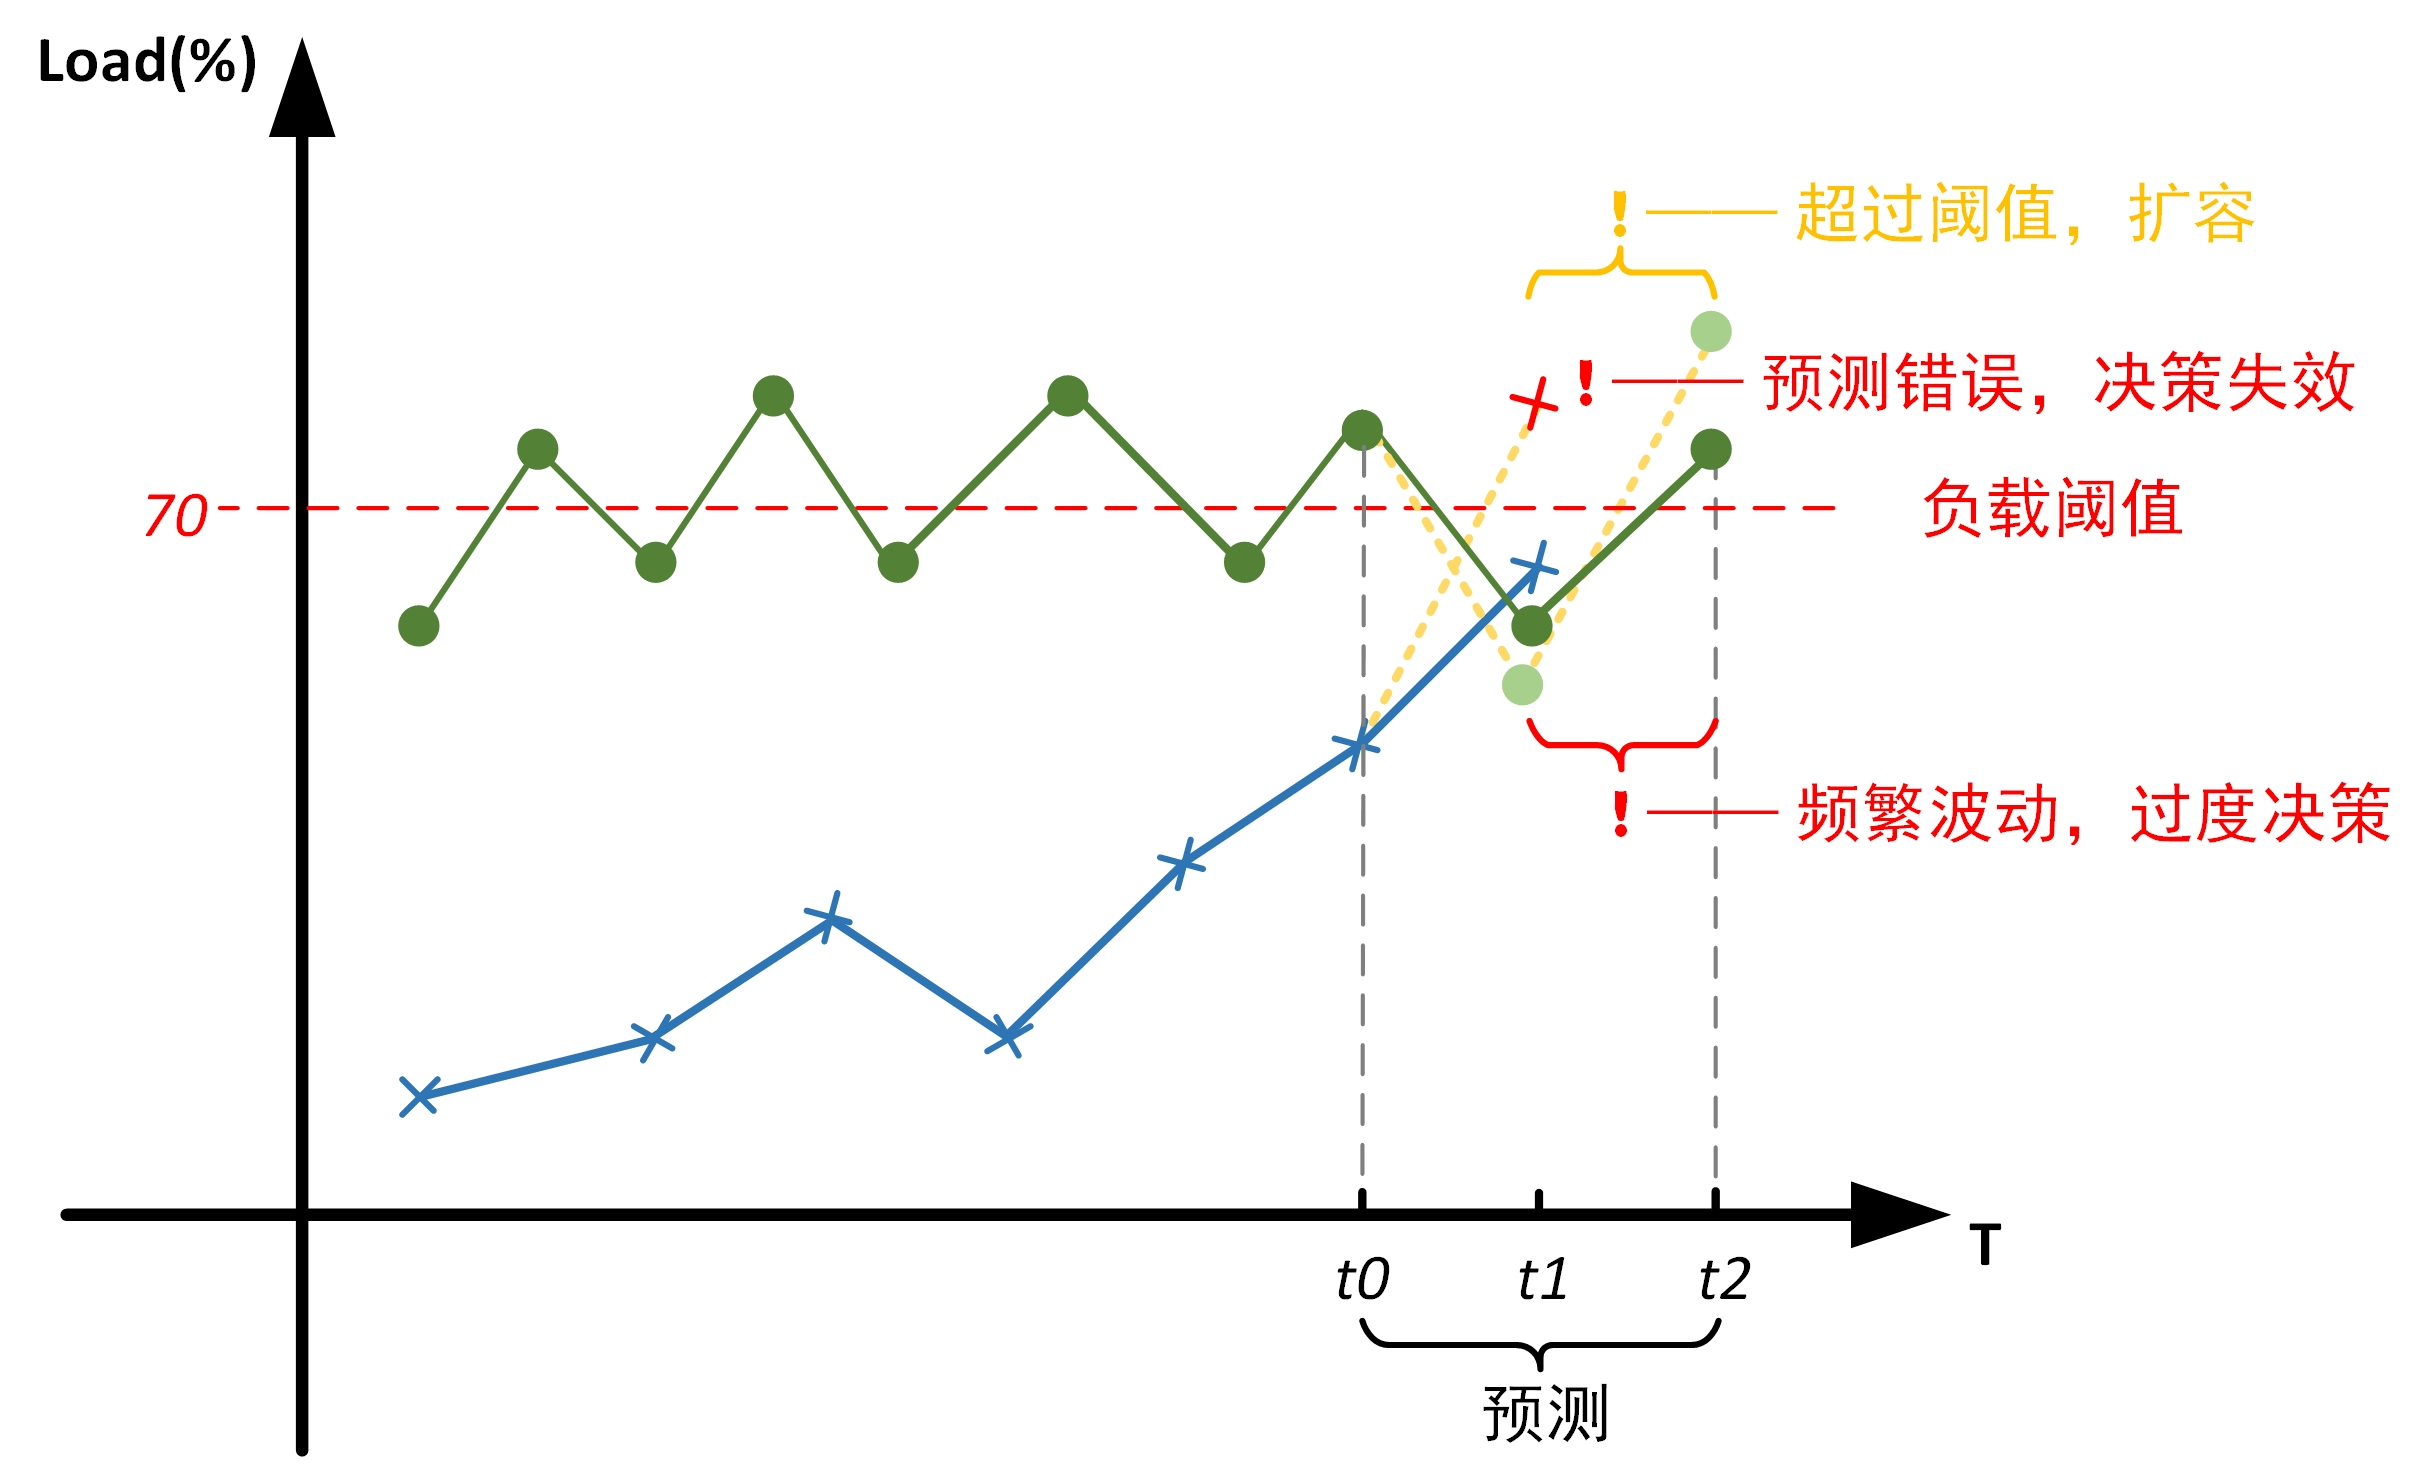
\includegraphics[scale=0.87]{figures/fig4_single_model.jpg}
\caption{单值预测模型}
\label{fig:fig4}
\end{figure}
}

\onslide*<4>{
\begin{figure}[htb]
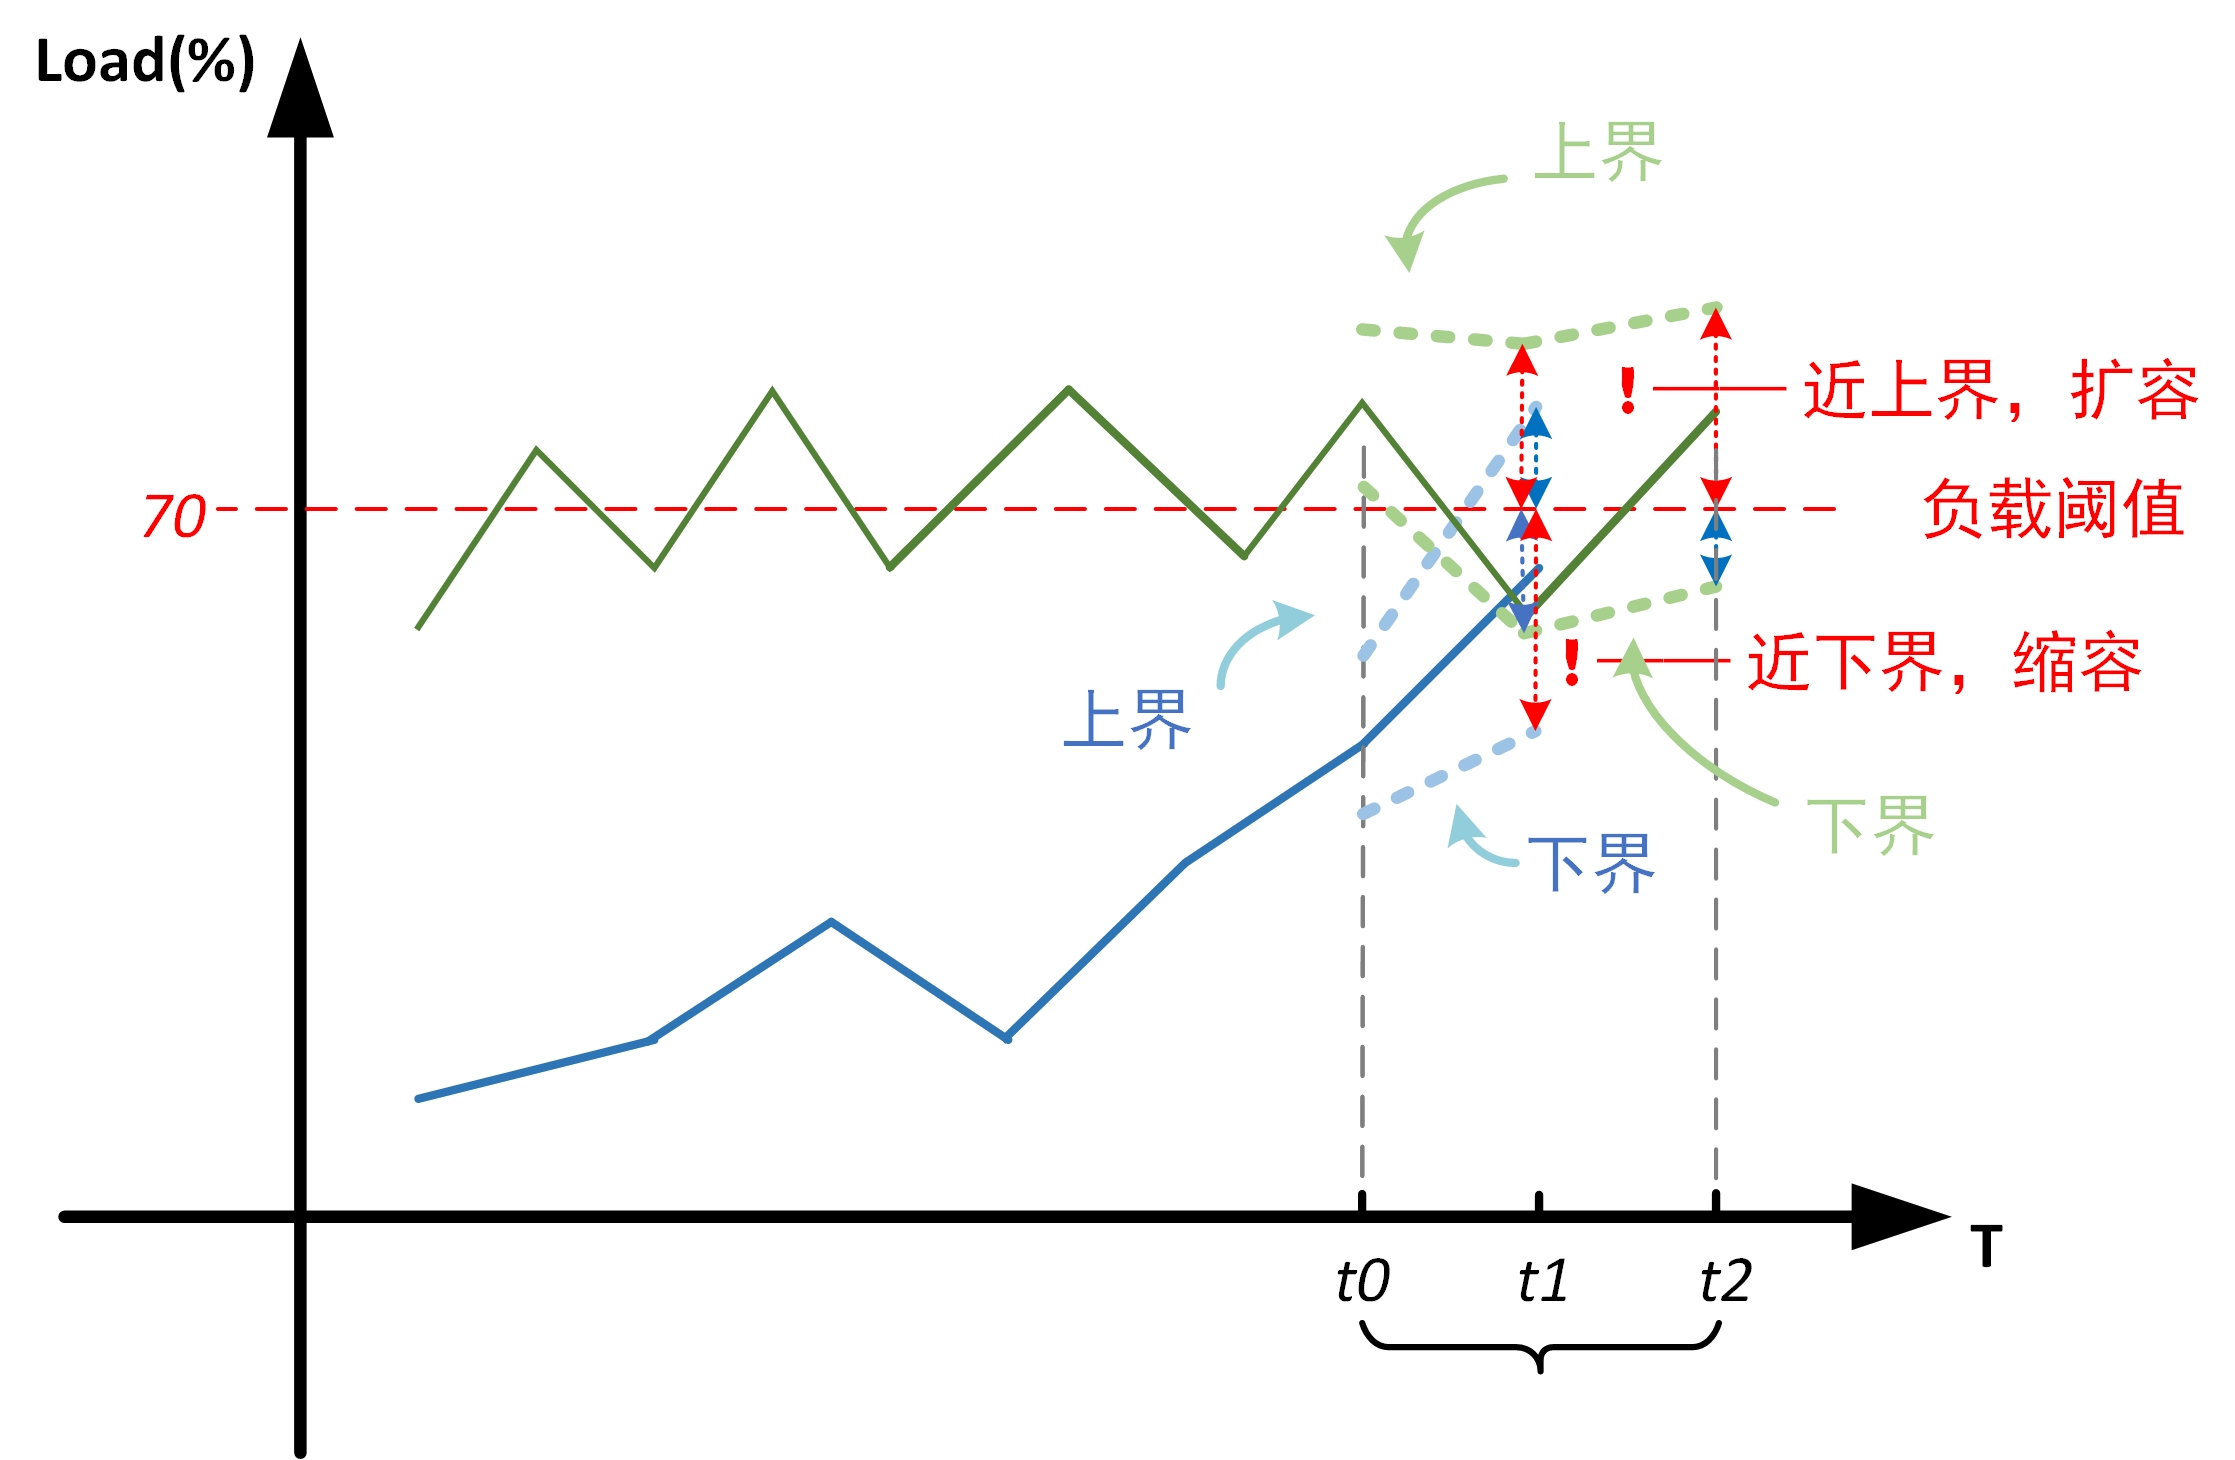
\includegraphics[scale=0.87]{figures/fig5_interval_model.jpg}
\caption{区间预测模型}
\label{fig:fig5}
\end{figure}
}
\end{frame}

\subsubsection{容器调度策略}

\begin{frame}
\frametitle{研究目标}
\framesubtitle{目标2:容器调度策略}
\begin{block}{容器调度策略:保证QoS同时降低能耗}
\begin{itemize}
    \item 动态调整容器数量:提高资源利用率
    \item 放置、迁移新增的和高负载主机上的容器:保证QoS
    \item 合并低负载主机上的容器:减少虚拟机和已激活服务器数量,避免不必要的能耗
\end{itemize}
\end{block}
\end{frame}